\documentclass{beamer}
\beamertemplatenavigationsymbolsempty
\usecolortheme{beaver}
\setbeamertemplate{blocks}[rounded=true, shadow=true]
\setbeamertemplate{footline}[page number]
%
\usepackage[utf8]{inputenc}
\usepackage[english,russian]{babel}
\usepackage{amssymb,amsfonts,amsmath,mathtext}
\usepackage{subfig}
\usepackage[all]{xy} % xy package for diagrams
\usepackage{array}
\usepackage{multicol}% many columns in slide
\usepackage{hyperref}% urls
\usepackage{hhline}%tables
% Your figures are here:
\graphicspath{ {fig/} {../fig/} }

%----------------------------------------------------------------------------------------------------------
\title[\hbox to 56mm{Задачи планирования}]{	Экспериментальное сравнение \\ задач оперативного планирования биохимического производства.}
\author[В.\,В. Пырэу]{Виталий Вячеславович Пырэу}
\institute{Московский физико-технический институт}
\date{\footnotesize
\par\smallskip\emph{Курс:} Автоматизация научных исследований\par (практика, В.\,В.~Стрижов)/Группа Б05-821
\par\smallskip\emph{Эксперт:} С.\,А.~Тренин
\par\bigskip\small 2021}
%----------------------------------------------------------------------------------------------------------
\begin{document}
%----------------------------------------------------------------------------------------------------------
\begin{frame}
\thispagestyle{empty}
\maketitle
\end{frame}

\begin{frame}{Цели исследования.}
\textbf{Основная решаемая задача}: получить оптимальное или качественное допустимое расписание для производства, используя как можно более простую модель.


\textbf{Цель исследования}: сравнить дискретный и непрерывный подходы к моделированию и описать классы задач, в которых модели, полученные в рамках каждого из подходов будут проще.

\textbf{Критерии качества}: число переменных и ограничений модели, производящей финальное расписание для процессов с различной STN-диаграммой
\end{frame}
\begin{frame}{Моделирование времени, ограничений и требований к расписанию}
\begin{enumerate}
	\item Дискретный индикатор времени $s_{i, t} = 1$ если задача $i$ началась в момент $t$.
	\item Прореживание сетки + сдвиг влево (только $t$ кратные $t_0$)
	\item Индикатор порядка задач: $b_{i, j} = 1$, если задача $i$ начинается раньше задачи $j$.
\end{enumerate}

\begin{center}
\includegraphics[width=0.7\textwidth]{Пример процесса}
\end{center}

\end{frame}

\begin{frame}{Литература}
	\begin{enumerate}
	\item \textbf{STN-диаграммы}: E. Kondili, С. C. Pantelidest and R. W. H. Sargent. A general algorithm for short-term scheduling of batch operations-i. MILP formulation
	\item \textbf{Обзор современных достижений}: Georgios P. Georgiadis, Apostolos P. Elekidis and Michael C. Georgiadis. Optimization-based scheduling for the process Industries: from theory to real-life Industrial applications.
	\item \textbf{Двухступенчатая схема}: F. Blomer, H.-O. Gunther. LP-based heuristics for scheduling chemical batch processes.
	\item \textbf{Схема, основанная на порядке}: C.A. Mendez, G.P. Henning, J. Cerda. An MILP continuous-time approach to short-term scheduling of resource-constrained multistage flowshop batch facilities.
\end{enumerate}
\end{frame}

\begin{frame}{Постановка задачи}
	Расписание должно быть оптимальным с точки зрения целевой функции - Makespan и учитывать следующие ограничения:
	\begin{enumerate}
	\item На конец производства выполнен весь заказ, то есть произведено как минимум столько продукта, сколько требовалось
	\item Склад не переполнен в течении всего времени производства
	\item Всякий процесс в расписании может взять со склада требуемый ему материал
	\item Один узел в каждый момент времени занимается не более, чем одной задачей.
\end{enumerate}
\end{frame}

\begin{frame}{Дискретная модель с плотным временем}
	\begin{enumerate}
	\item Переменные-индикаторы того, что процесс берёт задачу в некоторый момент
	\item Поток материала в каждый момент времени --- взвешанная сумма индикаторов
	\item Гарантируется получение оптимального расписания
	\item С удлинением временной шкалы число переменных резко возрастает даже при небольшом числе задач.
\end{enumerate}

\begin{center}
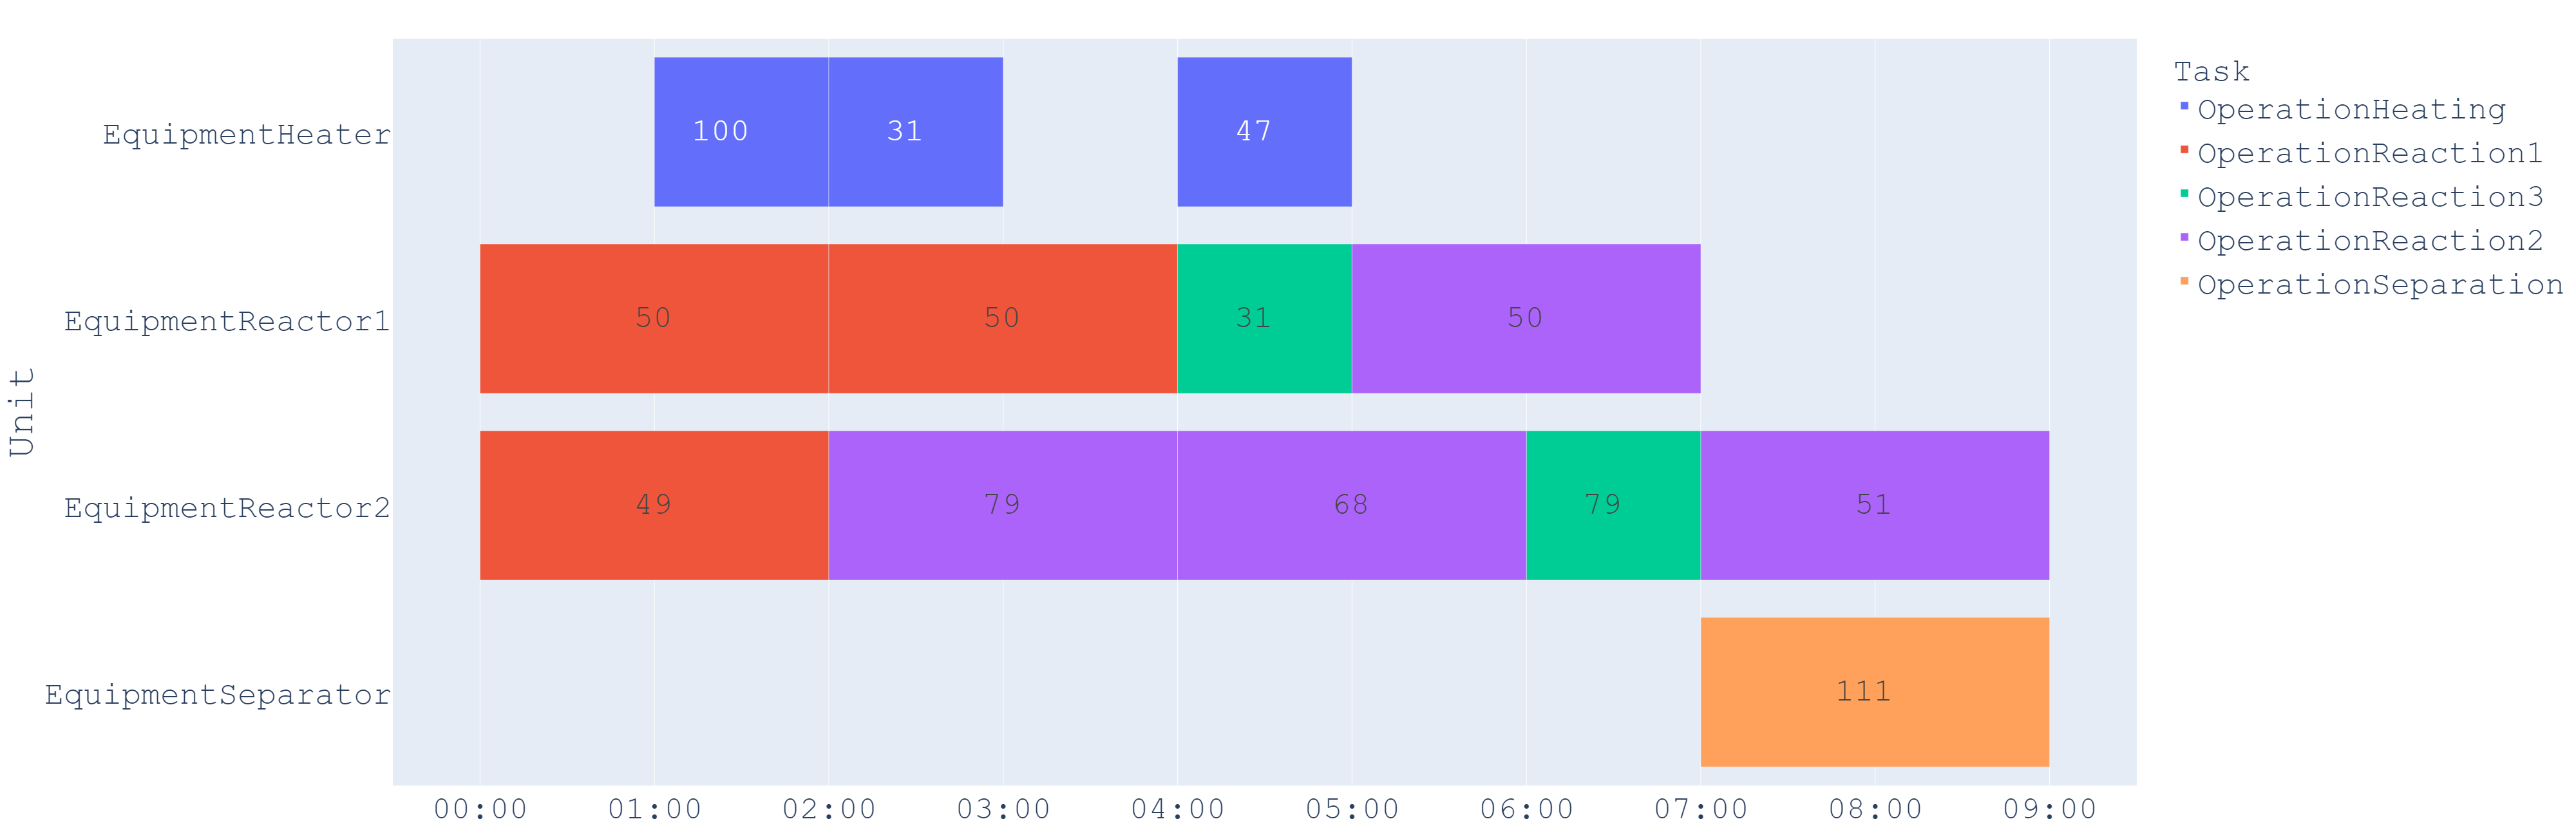
\includegraphics[width=1.0\textwidth]{plan}
\end{center}

\end{frame}

\begin{frame}{Двухступенчатая схема}
	\begin{enumerate}
	\item Решает проблему длинной временной шкалы
	\item Делит получение расписания на две фазы: грубое приближение и уточнение
	\item На первой фазе задачам разрешено начинаться только в малое число точек времени
	\item Не гарантирует получение оптимального расписания, но на практике даёт хорошее приближение сравнительно дёшево.
	\item Позволяет балансировать между сложностью модели и оптимальностью результата подбором плотности временной шкалы. Самая простая модель --- когда длина временных отрезков равна НОК длин процессов.
\end{enumerate}

\begin{center}
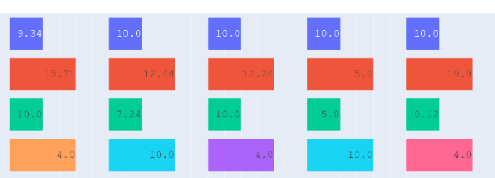
\includegraphics[width=1.0\textwidth]{plan sparsed}
\end{center}

\end{frame}

\begin{frame}{Схема, основанная на порядке}
	\begin{enumerate}
	\item Минимально моделирует временную шкалу
	\item Берёт во внимание не точное время событий, а их очерёдность
	\item Число переменных растёт квадратично от числа задач, но не зависит от плотности временной шкалы.
	\item Модели становятся более сложными, если процесс сетевой и простыми, если процесс линейный.
	
\end{enumerate}

\begin{center}
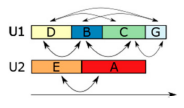
\includegraphics[width=0.5\textwidth]{precendance model}
\end{center}

\end{frame}

\begin{frame}{Итоги эксперимента}

	\begin{table}[50pt]
\centering
\renewcommand{\arraystretch}{2}
	\resizebox{\columnwidth}{!}{\begin{tabular}{ |c|c|c|c|c| }
		 \hline
		 Модель & Demand 500, время 50 & Demand 200, время 30 & Demand 50, время 10 & Общий случай \\ [0.5ex] 
		 \hline\hline
		 Дискретная & 1276/1859 & 776/1119 & 276/379 & $O(Tn)$ \\ 
		 \hline
		 Двухступенчатая & 276+1471/379+1589 & 176+767/231+841 & 151+829/194+854& $O(\frac{Tn}{L_{max}}) + O(n + Tn)$  \\
		 \hline
		 Порядковая & 41431/121494 & 11905/34890 & 1735/5070 & $O(n^2)$  \\
		 \hline
		\end{tabular}}
		\caption{Количество переменных и ограничений при разных подходах к построению модели.}
	\end{table}

\end{frame}

\begin{frame}{Заключение}
	\begin{enumerate}
	\item Модели были запущены на трех различных процессах при различных требованиях на заказ.
	\item Рассмотрен простой сетевой процесс, известная задача бенчмарка Westenberger and Kallrath (1994) и линейный процесс, исполняемый параллельно.
	\item Описаны классы задач, на которых методы показывают приемлимое для практики качество
	\item Двухступенчатая схема доведена до фреймворка и готовится к демонстрации.
	
\end{enumerate}

\end{frame}
%----------------------------------------------------------------------------------------------------------
\end{document} 